\chapter{Исследовательская часть}

В данном разделе приводятся примеры работы программного обеспечения. Кроме того, проводится эксперимент, в котором анализируется производительность программного обеспечения.

\section{Примеры работы программного обеспечения}

На рисунке \ref{img:example-start} показана волновая поверхность в положении равновесия, на риснуках \ref{img:example-first} и \ref{img:example-second} представлено образование волн в результате движения сферы, а на рисунке \ref{img:control-panel} --- окно панели управления.

\begin{figure}[H]
	\begin{center}
		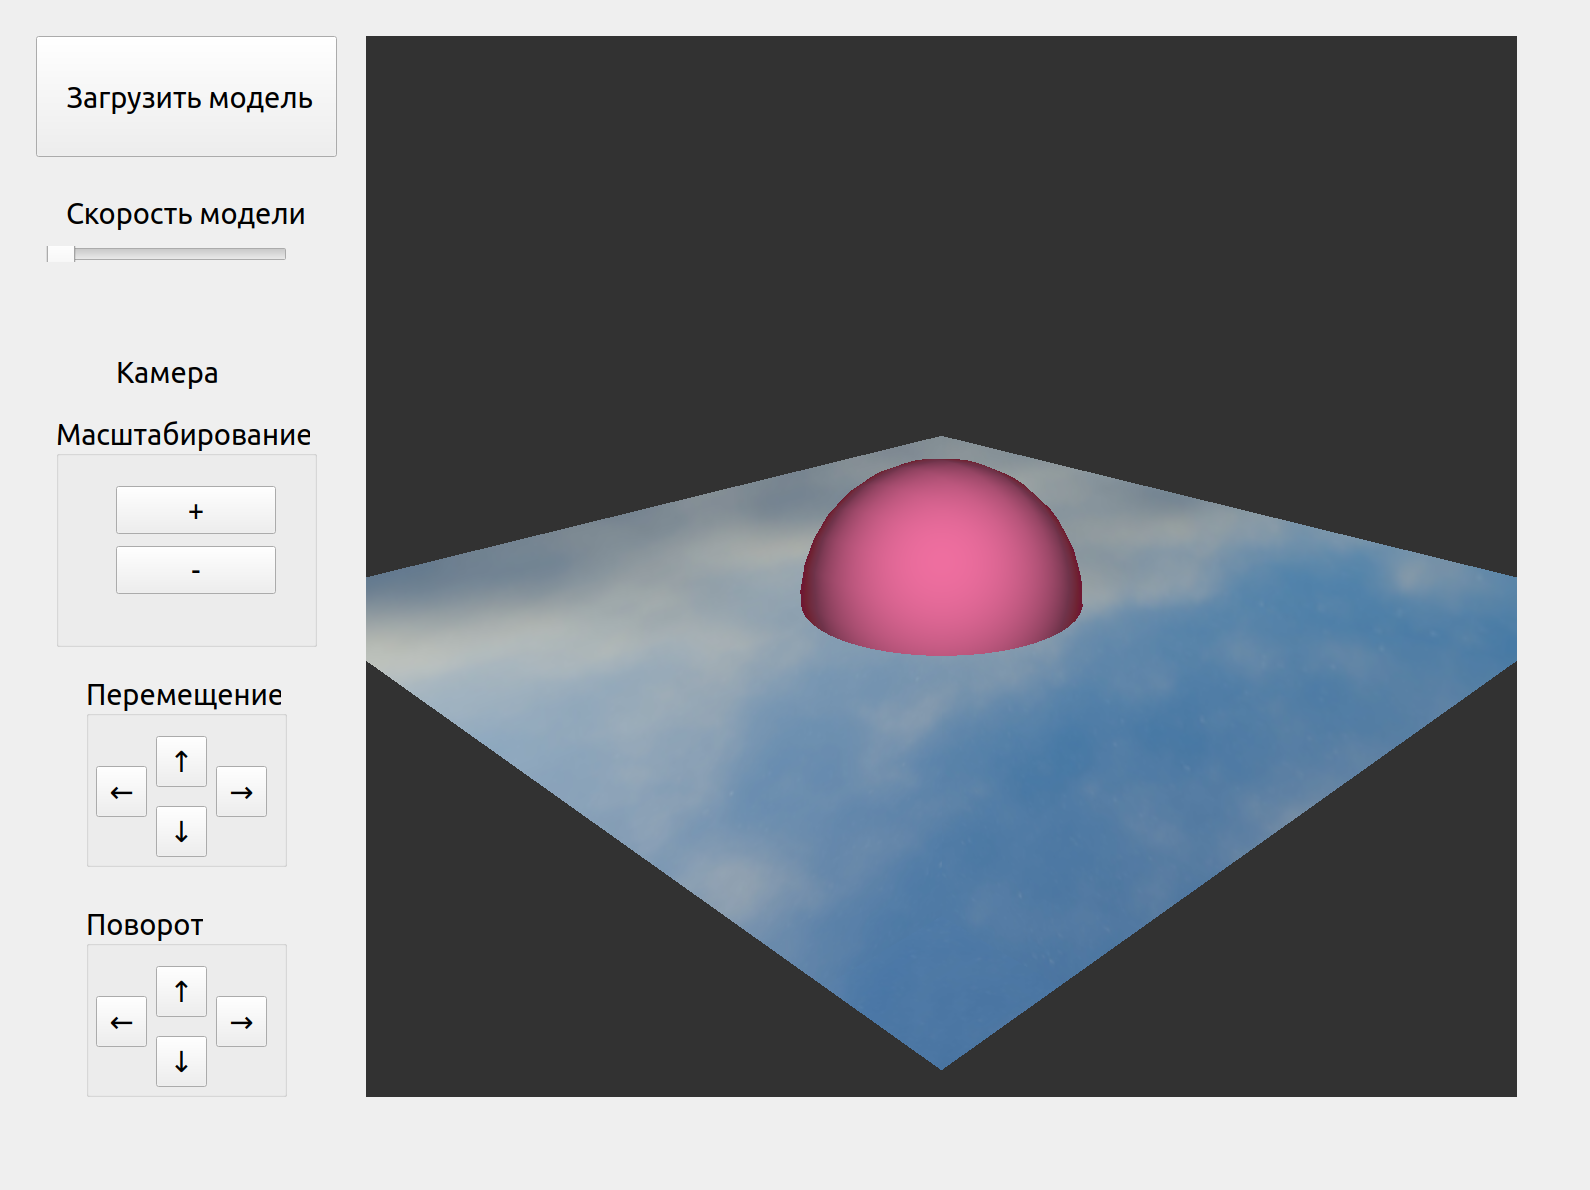
\includegraphics[scale=0.25]{img/example-start.png}
	\end{center}
	\captionsetup{justification=centering}
	\caption{Пример волновой поверхности в положении равновесия}
	\label{img:example-start}
\end{figure}

\begin{figure}[H]
	\begin{center}
		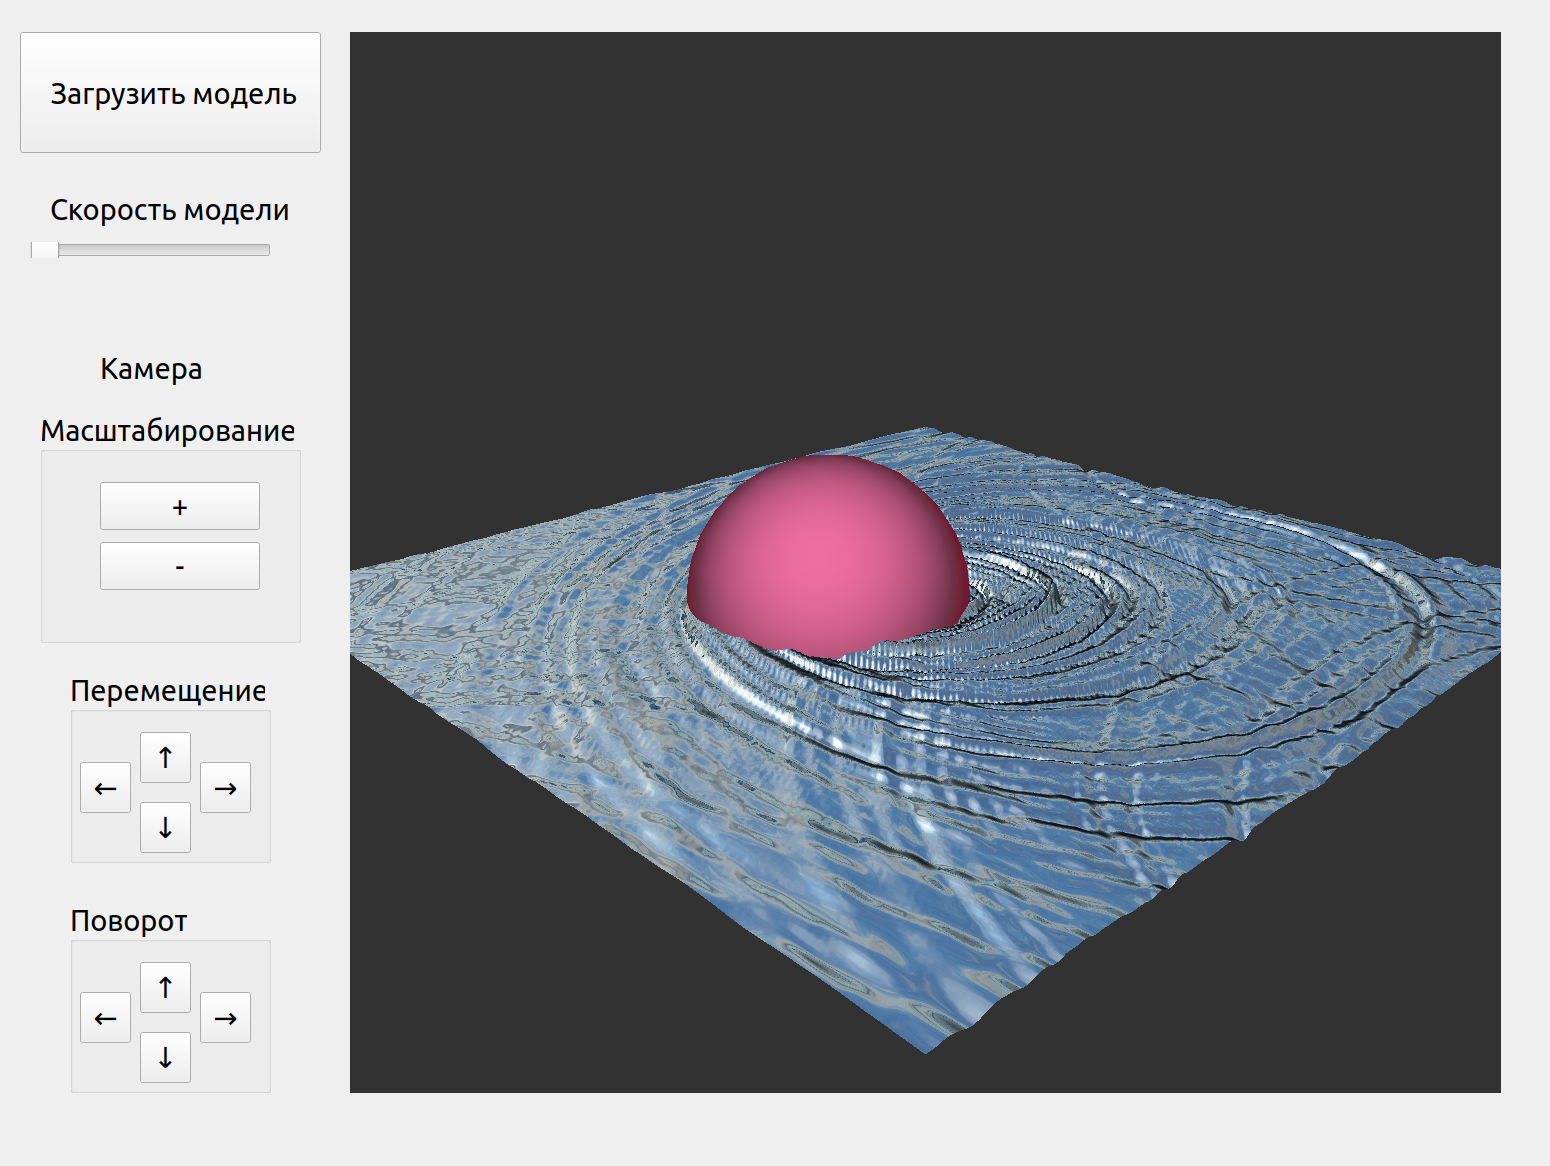
\includegraphics[scale=0.25]{img/example-first.png}
	\end{center}
	\captionsetup{justification=centering}
	\caption{Пример образования волн при движении сферы (вид 1)}
	\label{img:example-first}
\end{figure}

\begin{figure}[H]
	\begin{center}
		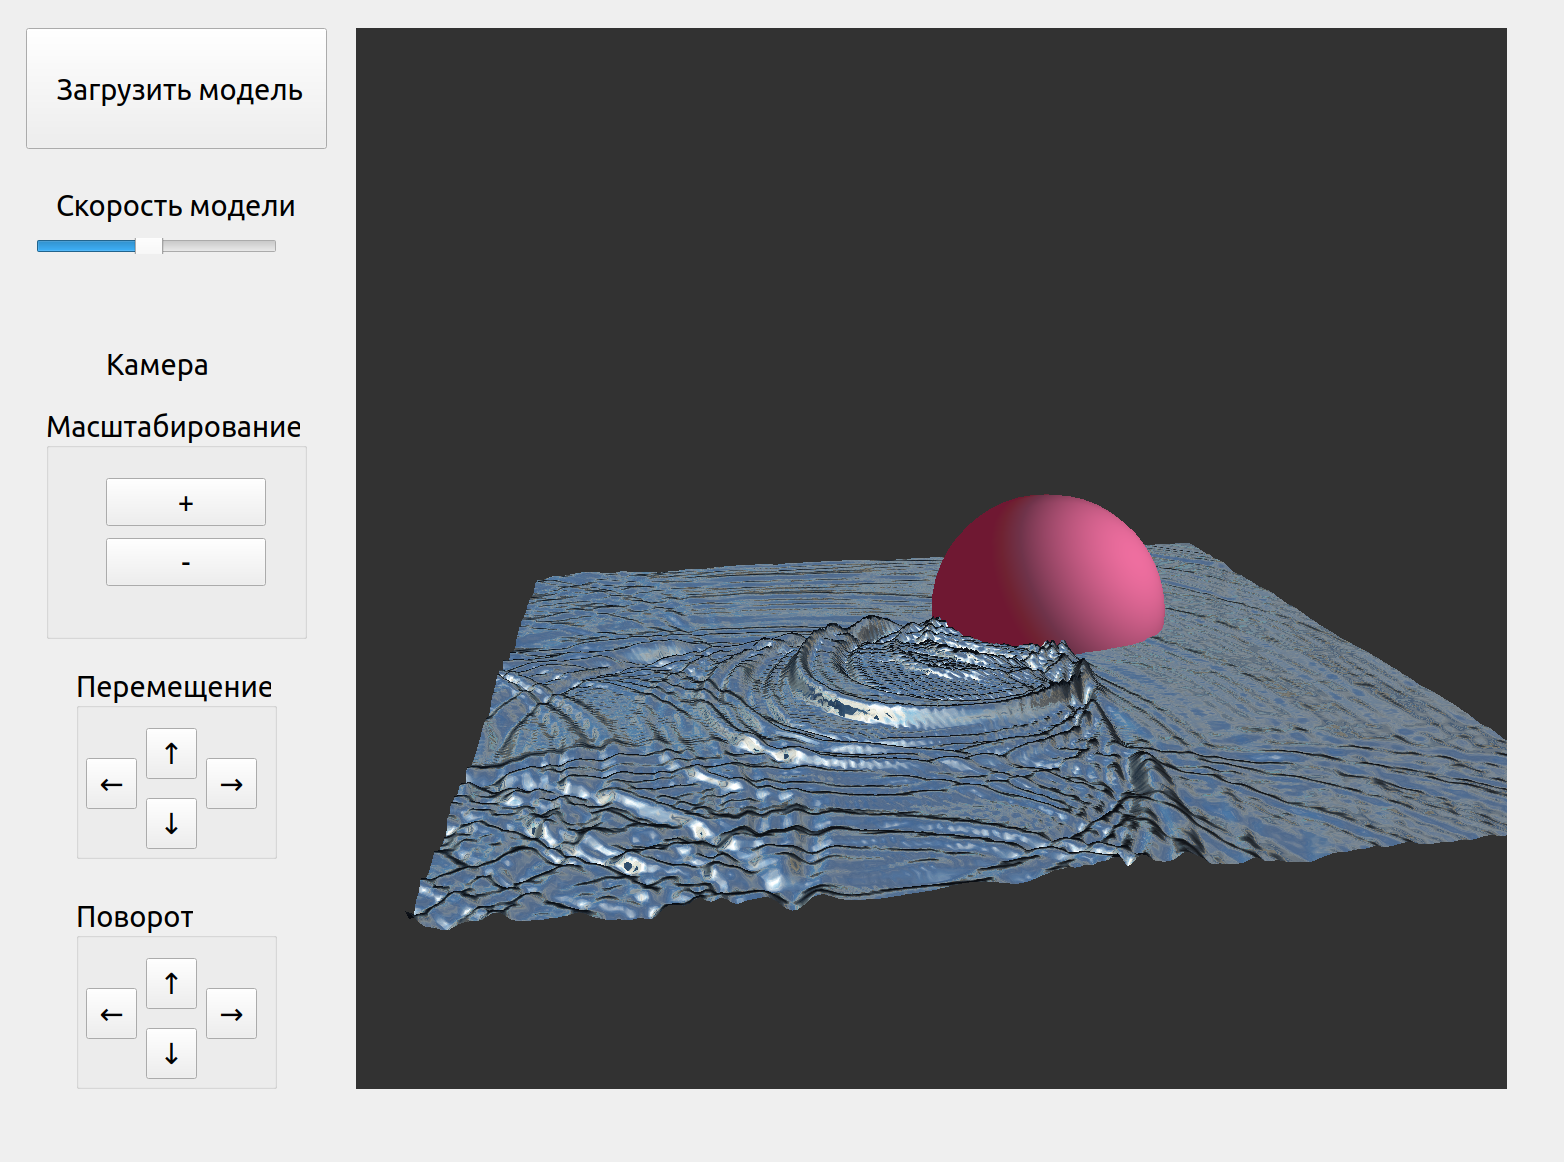
\includegraphics[scale=0.25]{img/example-second.png}
	\end{center}
	\captionsetup{justification=centering}
	\caption{Пример образования волн при движении сферы (вид 2)}
	\label{img:example-second}
\end{figure}

\begin{figure}[H]
	\begin{center}
		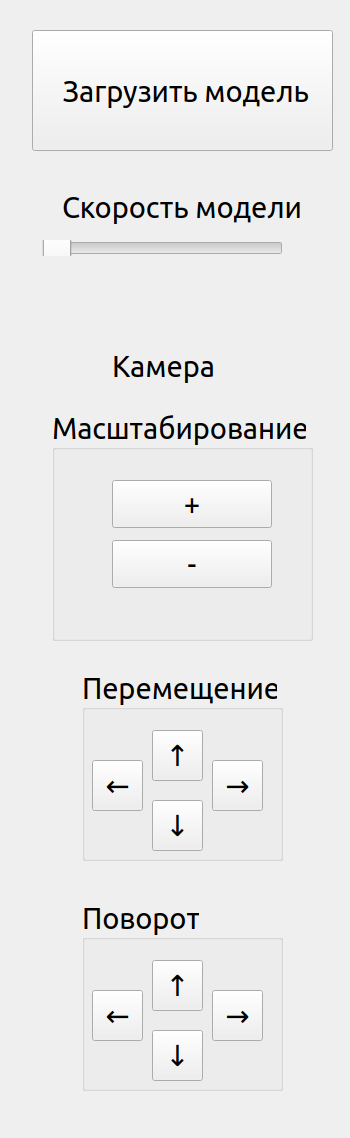
\includegraphics[scale=0.3]{img/control-panel.png}
	\end{center}
	\captionsetup{justification=centering}
	\caption{Окно панели управления}
	\label{img:control-panel}
\end{figure}

\section{Постановка эксперимента}